\documentclass{standalone}
\usepackage{tikz,tikz-3dplot}

\usetikzlibrary{math,shapes.geometric}

\begin{document}

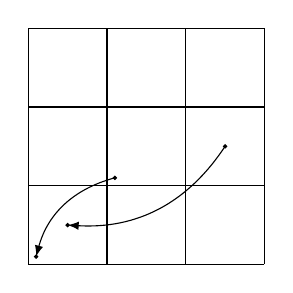
\begin{tikzpicture}
  \draw (0,0) grid (3,3);

  \coordinate (P) at (1.1,1.1);
  \coordinate (Q) at (0.1,0.1);
  \draw[fill=black] (P) circle[radius=0.02];
  \draw[fill=black] (Q) circle[radius=0.02];
  \draw[-latex] (P) to [bend right=30] (Q);

  \coordinate (P) at (2.5,1.5);
  \coordinate (Q) at (0.5,0.5);
  \draw[fill=black] (P) circle[radius=0.02];
  \draw[fill=black] (Q) circle[radius=0.02];
  \draw[-latex] (P) to [bend left=30] (Q);
\end{tikzpicture}

\end{document}